\section{Objetives}

The aim of this laboratory session is to analyze the basic components of polymer
matrix composites using physical-chemical techniques. For that matter,
Fourier Transform Infrared (FT-IR) is used.\\

\section{Materials}
In this experiment has been used an unsaturated polyester resin (UP), with
Methyl Ethyl Ketone Peroxide (MEKP), shown in figure \ref{fig:mekp}, as activator
of the curing process.\\

\begin{figure}[h]
	\centering
	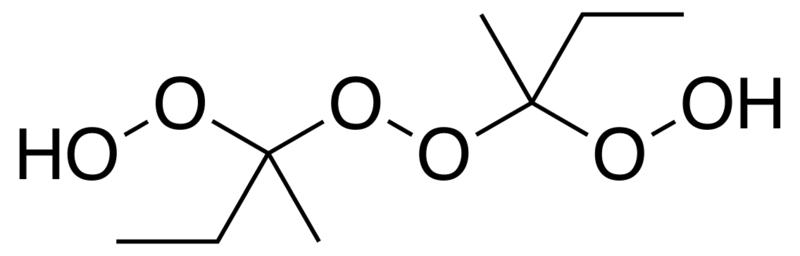
\includegraphics[width=0.5\textwidth]{img/MEKP.png}
	\caption{MEKP: Methyl Ethyl Ketone Peroxide chemical diagram}
	\label{fig:mekp}
\end{figure}

\section{Equipment and machinery}
To perform the Fourier Transform Infrared (FT--IR) spectroscopy, a spectrometer
such as a Nicolet Nexus 670 FTIR has been used (Figure \ref{fig:machinery}). For this experiment
has been used a mid-infrared region ($4000 \rightarrow 400 cm^{-1}$), as most organic compounds
and inorganic ions have its absorption radiation within this region.\\

\begin{figure}[h]
	\centering
	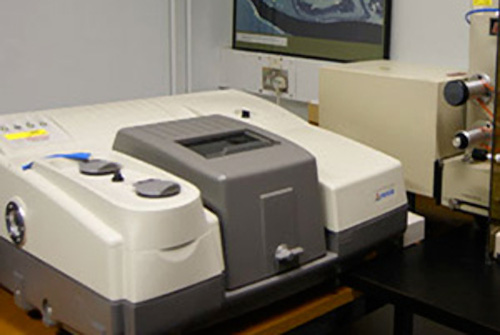
\includegraphics[width=0.5\textwidth]{img/machinery.jpg}
	\caption{A Nicolet Nexus 670 FTIR}
	\label{fig:machinery}
\end{figure}

\section{Experimental procedure}

For this experiment, Methyl Ethyl Ketone Peroxide (MEKP) is used as an activator
for the curing process of an unsaturated polyester resin (UP). A change of color can
be observed once the viscosity of the material starts to increase (changes from
blue to green).\\

To perform the measures on the FT-IR, a little sample of this viscous material
is placed between two salt plates. Salt crystals are used as they are “transparent”
and don’t tamper the results. Anyways, their spectrum has to be calculated previously
in order to erase it from the final results.\\

Measures can change depending on thickness and light path, that’s why is important
to avoid taking samples containing bubbles or large quantities of the samples.
During industrial production is also crucial to avoid bubbles forming inside the
material as they could worsen the material properties.\\

Once the material is placed inside the spectrometer, samples are taken every 2
minutes for a period of 14 minutes. Curing is accelerated during this process,
initially temperature is increased from 25 ºC (room temperature) to 40 ºC and
from then to a medium stage of 50 ºC and a final one of 60 ºC.\\

\section{Results and discussion}
The curing process can be done by mechanisms that do not produce any volatile
by-products and so are much easier to process, such as polyesters resins. Once
cured, thermosets will not be liquid again, though at a certain temperature,
their mechanical properties will change significantly. Increasing this temperature
we can also accelerate the curing process, as we have done on our experiment.
Above this certain temperature, $T_g$, the molecular structure changes from a rigid
state to a more flexible one and it is an irreversible process.\\

Polyester resins tend to be viscous, pale coloured liquids consisting of a solution
of a polyester in a monomer which is usually styrene. The addition of styrene performs
a vital function that is to enable the resin to cure from a liquid to a solid by
crosslinking the molecular chains of the polyester without the evolution of any
by-products. The styrene crosslinks the polymer chains at each of the reactive
sites to form a highly complex three-dimensional network.\\

The results of our experience shows that everything fits with the theory, and
furthermore, we are able to measure the curing percentage of our material. The complete
spectrum of the UP mixed with the peroxide and introduced between the salt crystals,
is shown in the figure \ref{fig:plot_full}, where the NaCl spectrum has been already
substracted. This plot corresponds with $t=0$, when we assume that curing process
hasn't yet started.\\

\begin{figure}[h]
	\centering
	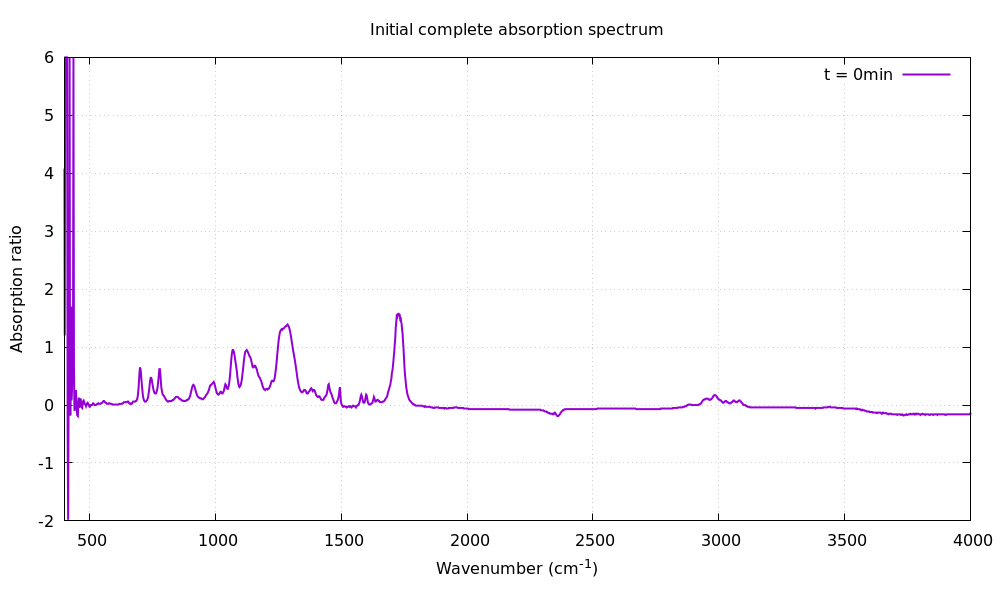
\includegraphics[width=\textwidth]{img/complete_spectrum.png}
	\caption{Full spectrum analyzed at $t = 0min$}
	\label{fig:plot_full}
\end{figure}

To quantify the curing process, multiple measures has been done each 2 minute intervals.
A closer look at the interesting range of data, for each time is shown in the next figure
\ref{fig:plot_full_zoom}:

\begin{figure}[h]
	\centering
	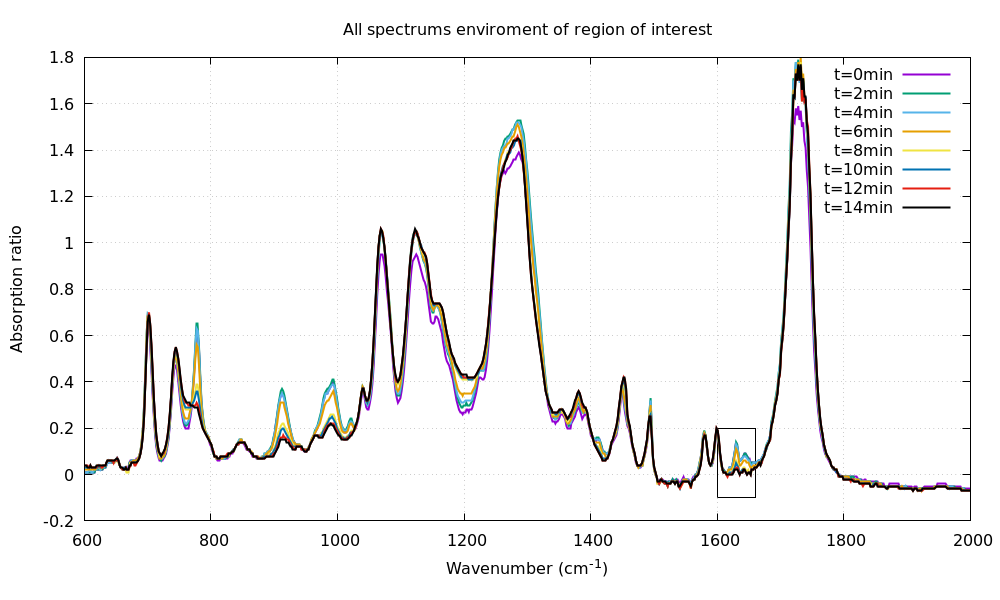
\includegraphics[width=0.8\textwidth]{img/complete_spectrum_zoom.png}
	\caption{A closer plot of the interesting frequency range for each time step}
	\label{fig:plot_full_zoom}
\end{figure}

Our region of interest corresponds with the frequency at the C=C double bond
vibrates, which is centered around $1630cm^{-1}$. Figure \ref{fig:cc_bond} is a zoomed
plot of the rectangle displayed in previous figure, and shows a decrease in the
absorption coefficient around this frequency. This could be interpreted as a
decrease in the total number of C=C double bonds, that is an indicator of the
creation of crosslinks.\\

\begin{figure}[h]
	\centering
	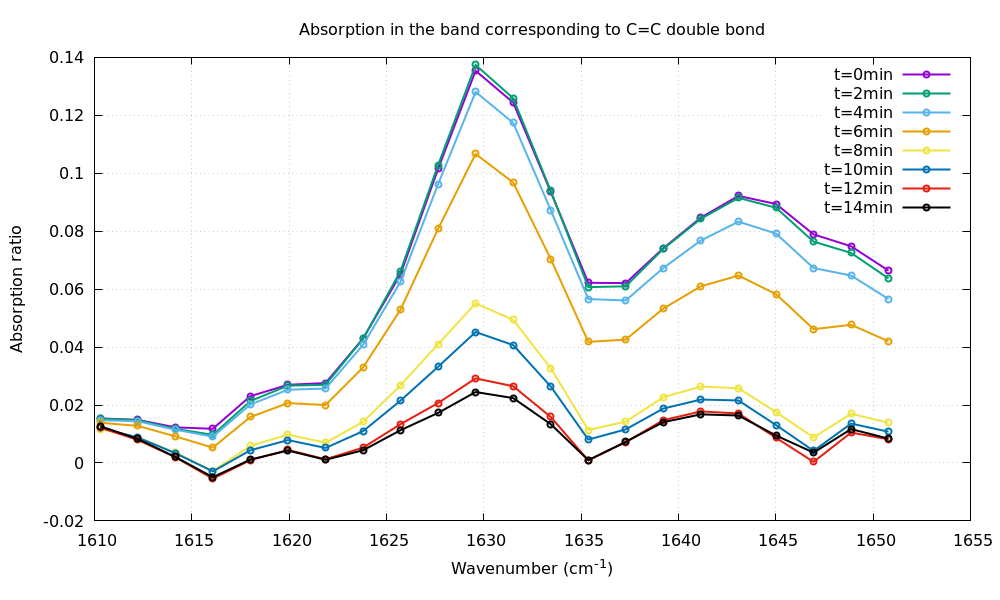
\includegraphics[width=0.9\textwidth]{img/cc_bond_dicrease.png}
	\caption{Enviroment of C=C double bond absorption band}
	\label{fig:cc_bond}
\end{figure}

To infer the percentage of curing we are assuming that at time zero, the curing
process is not started yet (curing percentage = 0\%), and the total disappearance
of double bonds would means a 100\% curing percentage. And to measure the
height of the peak we have calculated the height of the maximum value of the
peak from the base value, which is interpolated between the lateral
edges of the gaussian-like peak.

\begin{figure}[t]
	\centering
	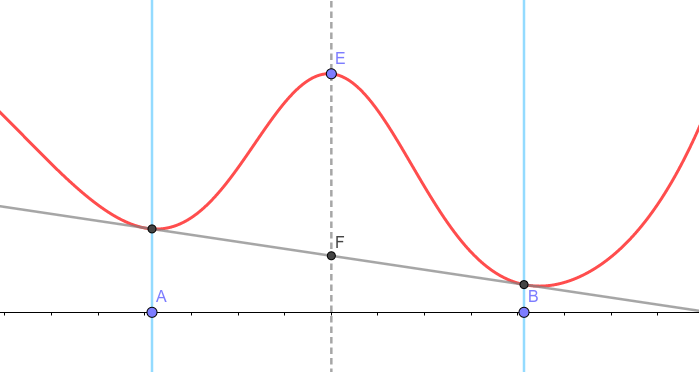
\includegraphics[width=0.4\textwidth]{img/calculation_peak_height.png}
	\caption{Method of calculating peak heights}
	\label{fig:calculation}
\end{figure}

According to diagram \ref{fig:calculation}, the height of the peaks (H) would be:

\begin{equation}
	H = y_E - y_F = y_E - \frac{y_B-y_A}{x_B-x_A} \left(x_E-x_A\right)
\end{equation}

And then, the curing percentage, C:

\begin{equation}
	C(\%) = 100 \left(1-\frac{H}{H_{max}}\right)
\end{equation}
where $H_{max}$ is the larger H of each time step.

After doing the calculations, we can plot the curing percentage for each time step
in the figure \ref{fig:curing_time}:

\begin{figure}[h]
	\centering
	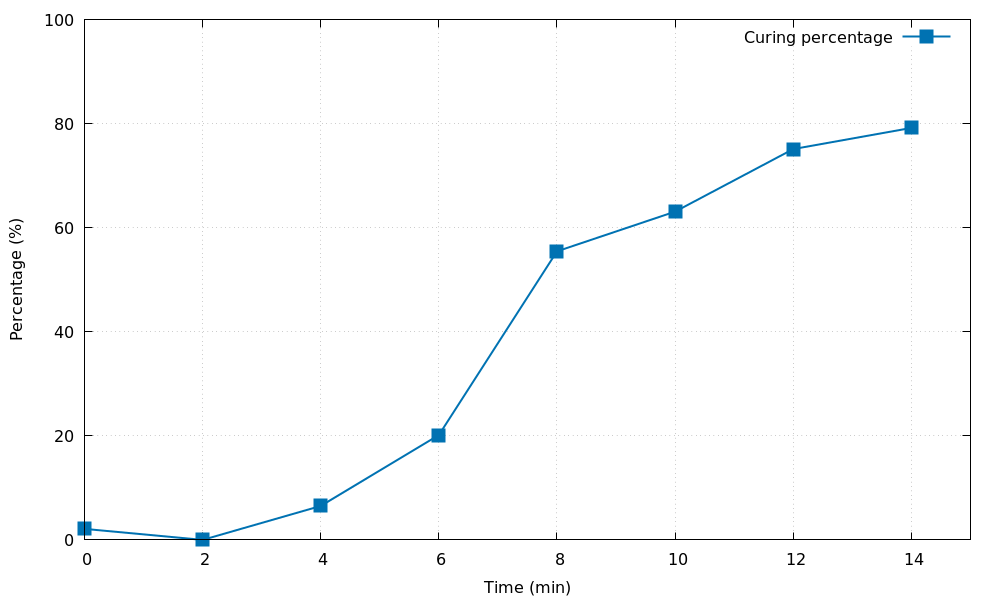
\includegraphics[width=0.7\textwidth]{img/curing_time.png}
	\caption{Curing percentage vs time}
	\label{fig:curing_time}
\end{figure}

We can compare our results with \cite{Canavate2000} where they used epoxy resin instead of polyester
resin but seeking the same results. They did heat the termoset, as we did, obtaining
similar results on the change of absortion of it, validating our results.\\

We can also compare our results with the ones from \cite{Jawad2016} where a process of heat
curing has been made as well. In this case they measured the transmitance of the
material, which is directly related with the absorbance under the equation:

\begin{equation}
	A = log_{10}\left(\frac{1}{T}\right)
\end{equation}

With different samples they showed the difference absorption in function of the
wave length dependent on the quantity of ZnO they added and the way of activating it.\\

As in our results, we can appreciate a different level of absorption dependent
not only on the change in proportion of materials but dependent on temperature.\\

Other comparisons have been made with our work in order to demonstrate the veracity
of our results. In the paper \cite{Nikolic2010} it has been done a crosslinked epoxy from a matrix
resin during 3 days. After that time there can be appreciated a change on the absorption
of the sample in function to the wavelength, (figure \ref{fig:epoxy}). We can refer to a specific
peak where it can be seen the epoxy peak for uncrosslinked resin (a) and the partially
crosslinked resin (b). We have something similar in our work where after a period
of time, though much less than the experiment \cite{Nikolic2010}, the absorbance changes depending
on the increase of temperature during time.\\

\begin{figure}[h]
	\centering
	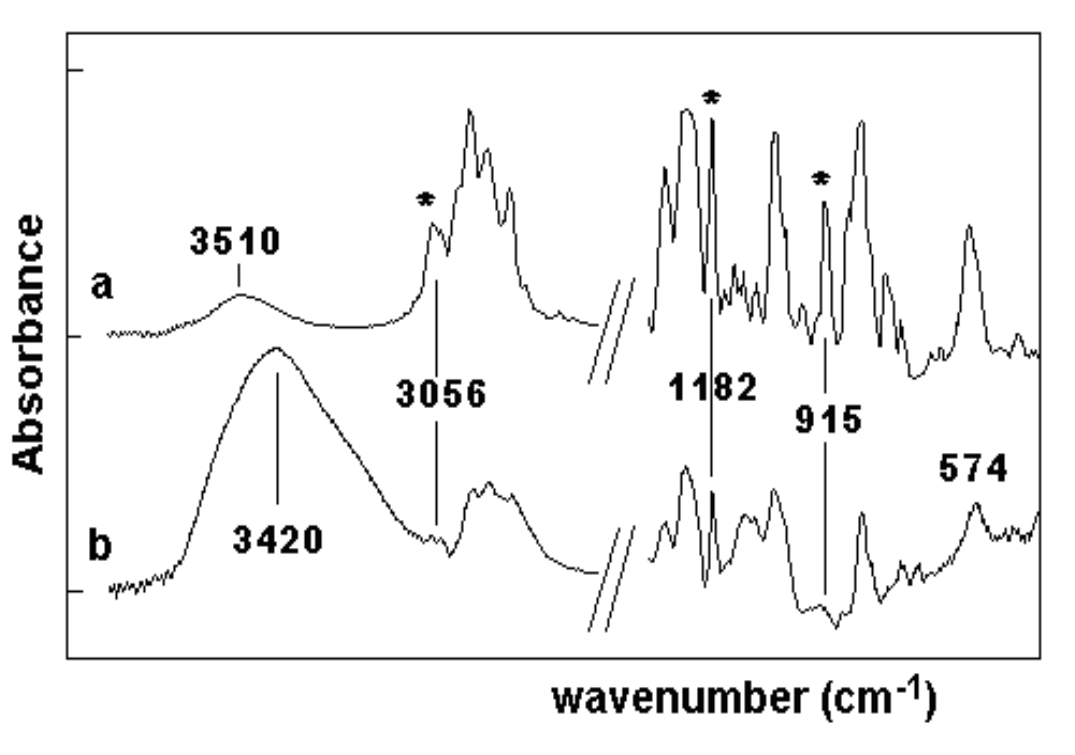
\includegraphics[width=0.65\textwidth]{img/crosslinked_epoxy.png}
	\caption{The partial FT-IR spectra of the unmodified GY250 resin (a) and the crosslinked
epoxy GY250/EH606/EH637 system after three days (b).}
	\label{fig:epoxy}
\end{figure}

\newpage

\vspace*{1px}

\section{Conclusion}

Results are as expected from theory, the addition of styrene reduces the double
bonds in function of the temperature thanks to the curing process, changing the
mechanical properties of the material.\\
